% questions.tex —— 2007 年·全国大纲卷Ⅱ·文科 · 题目内容片段（无答案）
% 由 tools/generate_projects.py 依来源总账自 2007/2007_数学真题_全国2文_试题.md 生成，勿手改（改源 MD 后重跑）


\gkpart{数学}

\begin{gktip}
\textbf{来源说明}：本题面依据固定源 PDF 两页 A3 题面逐题转录，原卷印刷页码 365–366。固定源不附答案，答案和解析均由本库独立复算；upstream 文件名按来源清单原样保留。

\textbf{图形说明}：第 20 题的原卷图形关系重绘为 TikZ/PGFPlots 矢量图。图形标记所指的 PNG 不随仓库保存。
\end{gktip}

\gkpart{一、选择题}

\begin{question}
\gkti{1}$\cos330^\circ=$\mbox{（　　）}

（A）$\dfrac12$\quad（B）$-\dfrac12$\quad（C）$\dfrac{\sqrt3}{2}$\quad（D）$-\dfrac{\sqrt3}{2}$

\end{question}
\begin{question}
\gkti{2}设全集 $U=\{1,2,3,4\}$，$A=\{1,2\}$，$B=\{2,4\}$，则 $\complement_U(A\cup B)=$\mbox{（　　）}

（A）$\{2\}$\quad（B）$\{3\}$\quad（C）$\{1,2,4\}$\quad（D）$\{1,4\}$

\end{question}
\begin{question}
\gkti{3}函数 $f(x)=|\sin x|$ 的一个单调递增区间是\mbox{（　　）}

（A）$\left(-\dfrac\pi4,\dfrac\pi4\right)$\quad（B）$\left(\dfrac\pi4,\dfrac{3\pi}4\right)$\quad（C）$\left(\pi,\dfrac{3\pi}2\right)$\quad（D）$\left(\dfrac{3\pi}2,2\pi\right)$

\end{question}
\begin{question}
\gkti{4}以下四个数中的最大者是\mbox{（　　）}

（A）$(\ln2)^2$\quad（B）$\ln(\ln2)$\quad（C）$\ln\sqrt2$\quad（D）$\ln2$

\end{question}
\begin{question}
\gkti{5}不等式 $\dfrac{x-2}{x+3}>0$ 的解集是\mbox{（　　）}

（A）$(-3,2)$\quad（B）$(2,+\infty)$\quad（C）$(-\infty,-3)\cup(2,+\infty)$\quad（D）$(-\infty,-2)\cup(3,+\infty)$

\end{question}
\begin{question}
\gkti{6}在 $\triangle ABC$ 中，已知 $D$ 是 $AB$ 边上一点，若 $\overrightarrow{AD}=2\overrightarrow{DB}$，$\overrightarrow{CD}=\dfrac13\overrightarrow{CA}+\lambda\overrightarrow{CB}$，则 $\lambda=$\mbox{（　　）}

（A）$\dfrac23$\quad（B）$\dfrac13$\quad（C）$-\dfrac13$\quad（D）$-\dfrac23$

\end{question}
\begin{question}
\gkti{7}已知正三棱锥的侧棱长是底面边长的 $2$ 倍，则侧棱与底面所成角的余弦值等于\mbox{（　　）}

（A）$\dfrac{\sqrt3}{6}$\quad（B）$\dfrac{\sqrt3}{4}$\quad（C）$\dfrac{\sqrt2}{2}$\quad（D）$\dfrac{\sqrt3}{2}$

\end{question}
\begin{question}
\gkti{8}已知曲线 $y=\dfrac{x^2}{4}$ 的一条切线的斜率为 $\dfrac12$，则切点的横坐标为\mbox{（　　）}

（A）$1$\quad（B）$2$\quad（C）$3$\quad（D）$4$

\end{question}
\begin{question}
\gkti{9}把函数 $y=e^x$ 的图象按向量 $\boldsymbol a=(2,0)$ 平移，得到 $y=f(x)$ 的图象，则 $f(x)=$\mbox{（　　）}

（A）$e^x+2$\quad（B）$e^x-2$\quad（C）$e^{x-2}$\quad（D）$e^{x+2}$

\end{question}
\begin{question}
\gkti{10}$5$ 位同学报名参加两个课外活动小组，每位同学限报其中的一个小组，则不同的报名方法共有\mbox{（　　）}

（A）$10$ 种\quad（B）$20$ 种\quad（C）$25$ 种\quad（D）$32$ 种

\end{question}
\begin{question}
\gkti{11}已知椭圆的长轴长是短轴长的 $2$ 倍，则椭圆的离心率为\mbox{（　　）}

（A）$\dfrac13$\quad（B）$\dfrac{\sqrt3}{3}$\quad（C）$\dfrac12$\quad（D）$\dfrac{\sqrt3}{2}$

\end{question}
\begin{question}
\gkti{12}设 $F_1,F_2$ 分别是双曲线 $x^2-\dfrac{y^2}{9}=1$ 的左、右焦点，若点 $P$ 在双曲线上，且 $\overrightarrow{PF_1}\cdot\overrightarrow{PF_2}=0$，则 $|\overrightarrow{PF_1}+\overrightarrow{PF_2}|=$\mbox{（　　）}

（A）$\sqrt{10}$\quad（B）$2\sqrt{10}$\quad（C）$\sqrt5$\quad（D）$2\sqrt5$

\end{question}
\gkpart{二、填空题}

\begin{question}
\gkti{13}一个总体含有 $100$ 个个体，以简单随机抽样方式从总体中抽取一个容量为 $5$ 的样本，则指定的某个个体被抽到的概率为\gkblank{}。

\end{question}
\begin{question}
\gkti{14}已知数列的通项 $a_n=-5n+2$，则其前 $n$ 项和为 $S_n=$\gkblank{}。

\end{question}
\begin{question}
\gkti{15}一个正四棱柱的各个顶点在一个直径为 $2\mathrm{cm}$ 的球面上。如果正四棱柱的底面边长为 $1\mathrm{cm}$，那么该棱柱的表面积为\gkblank{} $\mathrm{cm}^2$。

\end{question}
\begin{question}
\gkti{16}$(1+2x^2)\left(x+\dfrac1x\right)^8$ 的展开式中常数项为\gkblank{}。（用数字作答）

\end{question}
\gkpart{三、解答题}

\begin{question}
\gkti{17}设等比数列 $\{a_n\}$ 的公比 $q<1$，前 $n$ 项和为 $S_n$。已知 $a_3=2,S_4=5S_2$，求 $\{a_n\}$ 的通项公式。

\end{question}
\begin{question}
\gkti{18}在 $\triangle ABC$ 中，已知内角 $A=\dfrac\pi3$，边 $BC=2\sqrt3$，设内角 $B=x$，周长为 $y$。

（1） 求函数 $y=f(x)$ 的解析式和定义域；

（2） 求 $y$ 的最大值。

\end{question}
\begin{question}
\gkti{19}从某批产品中，有放回地抽取产品二次，每次随机抽取 $1$ 件，假设事件 $A$：“取出的 $2$ 件产品中至多有 $1$ 件是二等品”的概率 $P(A)=0.96$。

（1） 求从该批产品中任取 $1$ 件是二等品的概率 $p$；

（2） 若该批产品共有 $100$ 件，从中任意抽取 $2$ 件，求事件 $B$：“取出的 $2$ 件产品中至少有一件是二等品”的概率 $P(B)$。

\Needspace{0.4\textheight}
\end{question}
\begin{question}
\gkti{20}如图，在四棱锥 $S-ABCD$ 中，底面 $ABCD$ 为正方形，侧棱 $SD\perp$ 底面 $ABCD$，$E\text{、}F$ 分别是 $AB\text{、}SC$ 的中点。
\nopagebreak[4]
\begin{center}% 2007 年全国大纲卷Ⅱ文科第 20 题：正方形底面四棱锥
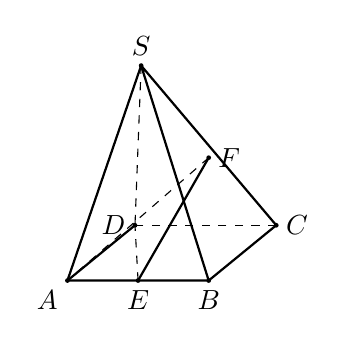
\begin{tikzpicture}[>=stealth,scale=0.78]
  \coordinate (A) at (0,0); \coordinate (B) at (2.3,0);
  \coordinate (C) at (3.4,0.9); \coordinate (D) at (1.1,0.9);
  \coordinate (S) at (1.2,3.5); \coordinate (E) at (1.15,0);
  \coordinate (F) at (2.3,2.0);
  \draw[thick] (A)--(B)--(C); \draw[dashed] (C)--(D); \draw[thick] (D)--(A);
  \draw[thick] (S)--(A) (S)--(B) (S)--(C);
  \draw[dashed] (S)--(D);
  \draw[thick] (E)--(F);
  \draw[dashed] (E)--(D) (F)--(A);
  \fill (S) circle (1.1pt) node[above] {$S$};
  \fill (A) circle (1.1pt) node[below left] {$A$};
  \fill (B) circle (1.1pt) node[below] {$B$};
  \fill (C) circle (1.1pt) node[right] {$C$};
  \fill (D) circle (1.1pt) node[left] {$D$};
  \fill (E) circle (1.1pt) node[below] {$E$};
  \fill (F) circle (1.1pt) node[right] {$F$};
\end{tikzpicture}
\end{center}
\nopagebreak[4]
（1） 求证：$EF\parallel$ 平面 $SAD$；

（2） 设 $SD=2CD$，求二面角 $A-EF-D$ 的大小。

\end{question}
\begin{question}
\gkti{21}在直角坐标系 $xOy$ 中，以 $O$ 为圆心的圆与直线 $x-3y=4$ 相切。

（1） 求圆 $O$ 的方程；

（2） 圆 $O$ 与 $x$ 轴相交于 $A,B$ 两点，圆内的动点 $P$ 使 $|PA|,|PO|,|PB|$ 成等比数列，求 $\overrightarrow{PA}\cdot\overrightarrow{PB}$ 的取值范围。

\end{question}
\begin{question}
\gkti{22}已知函数 $f(x)=\dfrac13 ax^3-bx^2+(2-b)x+1$ 在 $x=x_1$ 处取得极大值，在 $x=x_2$ 处取得极小值，且 $0<x_1<1<x_2<2$。

（1） 证明 $a>0$；

（2） 若 $z=a+2b$，求 $z$ 的取值范围。

\end{question}